\documentclass{article}
\usepackage[utf8]{inputenc}
\usepackage{graphicx} % Required for inserting images
\usepackage[a4paper, margin=1in]{geometry}
\usepackage[czech]{babel}
\usepackage{setspace}
\usepackage{adjustbox}

\usepackage{amsmath}
\usepackage{commath}
\usepackage{algorithm}
\usepackage{algorithmicx}

\begin{document}

% ÚVODNÍ STRÁNKA
\begin{titlepage}
    \centering
    \Large\textbf{Univerzita Karlova}
    
    \Large{Přírodovědecká fakulta}
    
    \vspace*{2.5cm}
    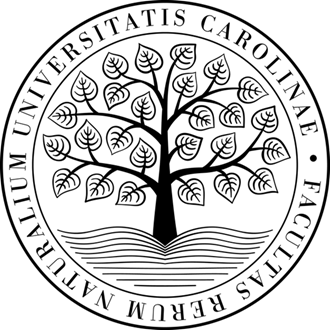
\includegraphics[width=0.55\linewidth]{images/prf.png}
    \vspace*{4cm}
    
    \Large\textbf{ALGORITMY POČÍTAČOVÉ KARTOGRAFIE}
    
    \Large{Digitální model terénu}
    
    \vspace*{3cm}
    \large Martina Pavlová, Martin Šíma, Ludmila Vítková

    1 N-GKDPZ
    
    Praha 2024
\end{titlepage}

% ZADÁNÍ
\begin{spacing}{1.5}
\section*{Zadání}

\noindent \emph {Vstup: množina P} $= \{p_1, \dots, p_n\}$, $p_i = \{x_i, y_i, z_i\}$.

\noindent \emph {Výstup: polyedrický \textbf{DMT} nad množinou $P$ představovaný vrstevnicemi doplněný vizualizací sklonu trojúhelníků a jejich expozicí.}.

\noindent Metodou inkrementální konstrukce vytvořte nad množinou P vstupních bodů 2D \emph{Delaunay triangulaci}. Jako vstupní data použijte existující geodetická data (alespoň 300 bodů) popř. navrhněte algoritmus pro generování syntetických vstupních dat představujících významné terénní tvary (kupa, údolí, spočinek, hřbet, \dots).

\noindent Vstupní množiny bodů včetně níže uvedených výstupů vhodně vizualizujte. Grafické rozhraní realizujte s využitím frameworku QT. Dynamické datové struktury implementujte s využitím STL.

\noindent Nad takto vzniklou triangulací vygenerujte polyedrický digitální model terénu. Dále proveďte tyto analýzy:

\begin{itemize}
  \item S využitím lineární interpolace vygenerujte vrstevnice se zadaným krokem a v zadaném intervalu, proveďte jejich vizualizaci s rozlišením zvýrazněných vrstevnic.
  \item Analyzujte sklon digitálního modelu terénu, jednotlivé trojúhelníky vizualizujte v závislosti na jejich sklonu.
  \item Analyzujte expozici digitálního modelu terénu, jednotlivé trojúhelníky vizualizujte v závislosti na jejich expozici ke světové straně.
\end{itemize}

\noindent Zhodnoťte výsledný digitální model terénu z kartografického hlediska, zamyslete se nad slabinami algoritmu založeného na 2D Delaunay triangulaci. Ve kterých situacích (různé terénní tvary) nebude dávat vhodné výsledky? Tyto situace graficky znázorněte.

\noindent Zhodnocení činnosti algoritmu včetně ukázek proveďte alespoň na 3 strany formátu A4.

\subsection*{\textbf{Hodnocení}}
\vspace{0.3cm}
\begin{adjustbox}{width=1\textwidth}
\begin{tabular}{|l|c|}
\hline
\textbf{Krok}                                                                                  & \textbf{hodnocení} \\ \hline
Delaunay triangulace, polyedrický model terénu.                                    &  10b              \\ \hline
Konstrukce vrstevnic, analýza sklonu a expozice                     & 10b    \\ \hline
\textit{Triangulace nekonvexní oblasti zadané polygonem} & \textit{+5b}    \\ \hline
\textit{Výběr barevných stupnic při vizualizaci sklonu a expozice}   & \textit{+3b}    \\ \hline
\textit{Automatický popis vrstevnic} & \textit{+3b} \\ \hline
\textit{Automatický popis vrstevnic respektující kartografické zásady (orientace, vhodné rozložení)}                    & \textit{+10b}    \\ \hline
\textit{Algoritmus pro automatické generování terénních tvarů (kupa, údolí, spočinek, hřbet, …)}                    & \textit{+10b}    \\ \hline
\textit{3D vizualizace terénu s využitím promítání}                    & \textit{+10b}    \\ \hline
\textit{Barevná hypsometrie}                    & \textit{+5b}    \\ \hline
\textbf{Max celkem:}                                                                                  & \textbf{65b} \\ \hline
\end{tabular}
\end{adjustbox}

\vspace{0.2cm}
\noindent V rámci této úlohy byla zpracována bonusová úloha triangulace nekonvexní oblasti.
\newpage

\section{Popis a rozbor problému }
Digitální model terénu je matematické zobrazení povrchu země, kde je pro libovolný bod modelu možné určit jeho nadmořskou výšku. Jsou v něm zahrnuty i terénní rysy, kterými jsou například kopce, údolí a~další topografické prvky. Jako podkladová data mohou být použita data získaná pomocí LIDARu nebo fotogrammetrie. Ke zpřesnění modelů lze použít satelitní snímky nebo letecké fotografie. Digitální model terénu lze využít pro vizualizaci a analýzu zemského povrchu ve 3D například pro plánování staveb silnic a mostů, k ochraně přírody nebo pro modelování povodní a půdní eroze. 

Často používanou metodou tvorby digitálního modelu terénu je TIN neboli \textit{Triangular Irregular Network}. Tyto modely jsou vytvářeny za pomoci sítě trojúhelníků, které vzniknou na základě vstupní bodové vrstvy. Pro každý bod počítá TIN nadmořskou výšku za použití interpolace výšek okolních bodů. Výška bodu je tedy odhadnuta přesněji na rozdíl od modelů, které například využívají pravidelné sítě nebo vrstevnice. V oblastech s dynamičtějšími změnami lze vytvořit více trojúhelníků různých velikostí a tím pádem dojde k lepšímu přizpůsobení nepravidelnému tvaru terénu. Mimo informace o nadmořské výšce zachycuje tento model i informace o sklonu terénu.

\subsection{Delaunay triangulace}
Jednou z nejčastěji používaných metod triangulace je Delaunay triangulace. Tuto triangulace lze tvořit nejen ve 2D, ale i ve 3D prostoru. V rámci této metody jsou vytvořeny trojúhelníky tak, aby byly co nejvíce rovnostranné. Tím dochází k minimalizaci případné deformaci trojúhelníků. Snaží se tedy maximalizovat minimální vnitřní úhel, čímž vzniká pravidelnější síť. Jednou z jejích vlastní je, že uvnitř kružnice opsané libovolnému trojúhelníku neleží žádný jiný bod za zadané vstupní množiny $P$.

Do vytvořené Dalaunay triangulace se postupně ukládají jednotlivé body, přičemž nejprve je ze vstupní množiny vybrán náhodný bod $P_1$. Na základě Eukleidovské vzdálenosti dojde k určení bodu $P_2$ jemu nejbližšímu. Z těchto dvou bodů vznikne hrana $e = (P_1, P_2)$. Dalším krokem je hledání bodu \textit{$\underbar{P}$}, který se vůči vzniklé hraně e nachází v levé polorovině. Tento bod zároveň minimalizuje poloměr kružnice opsané hraně e a tomuto bodu. Po nalezení tohoto bodu dochází ke vzniku dvou nových hran $e_2 = (\textit{\underbar{P}}, P_1)$ a $e_3 = (P_2, \textit{\underbar{P}})$. Vniklé hrany tvoří trojúhelník. V případě, že bod \textit{$\underbar{P}$} nebyl nalezen, dojde k~otočení orientace hrany $e$ a následuje opět hledání bodu v levé polorovině.

Všechny nově vytvořené hrany jsou následně přidány do \textit{Active Edges List (AEL)} a tvoří výslednou triangulaci. AEL obsahuje hrany $e$ pro které jsou hledány body \textit{$\underbar{P}$}. Po vyprázdnění tohoto seznamu dojde k vytvoření Delaunay triangulace. 

\newpage

\subsubsection*{Implementace Delaunay triangulace}
\begin{algorithm}[h]
    \caption {\textit{Delaunay triangulace}}
    \begin{algorithmic}[1]
        \State Inicializuj prázdný seznam $dt$
        \State Inicializuj prázdný seznam$ ael$
        \State Najdi bod $P_1$ s nejmenší x-ovou souřadnicí
        \State Najdi bod $P_2$, který je nejblíže bodu $P_1$
        \State Vytvoř z bodů $P_1$ a $P_2$ hranu $e$
        \State Vytvoř opačnou hranu $e\_op$ z bodů $P_2$ a $P_1$
        \State Přidej hranu $e$ do $ael$
        \State Přidej hranu $e\_op$ do $ael$
        \State Dokud není $ael$ prázdná
        \State \indent Vezmi první hranu $e1$ a otoč její orientaci
        \State \indent Najdi k této hraně Delaunayovský bod $p\_dt$
        \State \indent Pokud existuje $pq\_dt$
        \State \indent \indent Vytvoř hranu $e2$ z bodů e2\_op a p\_dt
       \State \indent \indent Vytvoř hranu $e3$ z bodů $pq\_dt$ a $e1$
       \State \indent \indent Vzniklé hrany přidej do $dt$
       \State \indent \indent Aktualizuj $ael$ 
        \State Vrať $dt$
    \end{algorithmic}
\end{algorithm}

\subsection{Konstrukce vrstevnic}
Pomocí lineární interpolace lze konstruovat vrstevnice tak, že jsou lineárními funkcemi prokládány křivky. Pokud máme zadané souřadnice dvou bodů $x_a$ a $y_a$, pak je lineární interpolací přímka mezi těmito dvěma body. Rovnici vzájemných vztahů můžeme odvodit z podobnosti trojúhelníků.

$$ x_a = \frac{x_3 - x_1}{z_3 - z_1}(z - z_1) + x_1 \indent \indent
x_b = \frac{x_2 - x_1}{z_2 - z_1}(z - z_1) + x_1 $$

$$ y_a = \frac{y_3 - y_1}{z_3 - z_1}(z - z_1) + y_1 \indent \indent
y_b = \frac{y_2 - y_1}{z_2 - z_1}(z - z_1) + y_1 $$

Principem této metody je hledání průsečnic roviny určené trojúhelníkem z Delaunay triangulace a~vodorovné roviny $\rho$, která má výšku $h$. Pomocí následující nerovnice lze určit, zda rovina $\rho$ prochází hranou tvořenou zadanými body.

$$(z - z_i)(z - z_{i+1}) < 0$$

\newpage

\subsubsection*{Implementace}
\begin{algorithm}[h]
    \caption {\textit{Vrstevnice}}
    \begin{algorithmic}[1]
        \State Inicializuj prázdný seznam $contours$
        \State Projdi všechny trojúhelníky v $dt$
        \State \indent Získej vrcholy trojúhelníku $P_1$, $P_2$, $P_3$ 
        \State \indent Získej z-ovou souřadnici vrcholů $P_1$, $P_2$, $P_3$ 
        \State \indent Projdi všechny hodnoty od $zmin$ do $zmax$ s krokem $dz$
       \State \indent \indent Vypočítej rozdíl mezi aktuální hodnotou $z$ a z-ovými souřadnicemi vrcholů trojúhelníku 
       \State \indent \indent Pokud jsou všechny vrcholy na stejné z-ové úrovni
       \State \indent \indent \indent Pokračuj
       \State \indent \indent Pokud jsou dvě hrany kolineární
       \State \indent \indent \indent Přidej trojúhelník do seznamu vrstevnic 
       \State \indent \indent Pokud jsou hrany trojúhleníku protínány rovinou dané z-ové souřadnice
       \State \indent \indent \indent Vypočítej průsečíky
       \State \indent \indent \indent Vytvoř nové hrany 
       \State \indent \indent \indent Přidej hranu do $contours$
        \State Vrať $contours$
    \end{algorithmic}
\end{algorithm}

\subsection{Analýza sklonu terénu}
Výpočet sklonu je proveden pro každý trojúhelník Delaunay triangulace. Pro rovinu $\rho$, jejíž obecná rovina vypadá následovně: 
$$\rho: ax +by + cz + d = 0$$

je vypočítán gradient $\nabla \rho$, neboli maximální vektor spádu. Tento gradient má v daném bodě směr normály k vrstevnici a zároveň je orientován ve směru funkce $p$.

$$\nabla \rho (x_0 , y_0 , z_0) = \left(\frac{\partial p}{\partial x}(x_0), \frac{\partial p}{\partial y}(y_0), \frac{\partial p}{\partial z}(z_0)  \right) = (a,b,c)$$

V případě, že máme vodorovnou rovinu $\pi$, pak mají roviny $\rho$ a $\pi$ normálové vektory $n_1$, $n_2$. Pro rovinu $\pi$ uvažujeme s jednotkovým vektorem
$$n_1 = (a, b, c), \ \  \ \  n_2 = (0, 0, 1)$$

Odchylku $\varphi$ od rovin $\rho$ a $\pi$ lze vypočítat ze vztahu: 

$$\varphi = arccos \frac{n_1 \cdot n_2}{\norm {n_1}\norm {n_2}} = arccos \frac{c}{\norm {n_1}} $$

\newpage
\subsubsection*{Implementace}
\begin{algorithm}[h]
    \caption {\textit{Sklon terénu}}
    \begin{algorithmic}[1]
        \State Vypočítej rozdíl x-ových souřadnic bodů $P_1$ a $P_2$
        \State Vypočítej rozdíl y-ových souřadnic bodů $P_1$ a $P_2$
        \State Vypočítej rozdíl z-ových souřadnic bodů $P_1$ a $P_2$
        \State Vypočítej rozdíl x-ových souřadnic bodů $P_1$ a $P_2$
        \State Vypočítej rozdíl y-ových souřadnic bodů $P_1$ a $P_2$
        \State Vypočítej rozdíl z-ových souřadnic bodů $P_1$ a $P_2$
        \State Vypočítej x-ovou souřadnici normálového vektoru trojúhelníku
        \State Vypočítej y-ovou souřadnici normálového vektoru trojúhelníku
        \State Vypočítej z-ovou souřadnici normálového vektoru trojúhelníku
        \State Vypočítej normu normálového vektoru
        \State Vrať hodnotu úhlu mezi normálovým vektorem a osou z
    \end{algorithmic}
\end{algorithm}


\subsection{Analýza orientace terénu}
Expozici neboli orientaci terénu lze definovat jako azimut průmětu gradientu $\nabla \rho$ do roviny $x$, $y$. Vznikne tedy vektor $\vec{v}$ s nulovou složkou $z$.

$$\vec{v} = \left(\frac{\partial p}{\partial x}(x_0), \frac{\partial p}{\partial y}(y_0), 0 \right) = (a,b,0)$$

Azimut tohoto vektoru je měřen od osy $y$ a lze vypočítat pomocí vztahu: 

$$A = arctan (\frac{a}{b})$$


\subsubsection*{Implementace}
\begin{algorithm}[h]
    \caption {\textit{Orientace terénu}}
    \begin{algorithmic}[1]
        \State Vypočítej rozdíl x-ových souřadnic bodů $P_1$ a $P_2$
        \State Vypočítej rozdíl y-ových souřadnic bodů $P_1$ a $P_2$
        \State Vypočítej rozdíl z-ových souřadnic bodů $P_1$ a $P_2$
        \State Vypočítej rozdíl x-ových souřadnic bodů $P_1$ a $P_2$
        \State Vypočítej rozdíl y-ových souřadnic bodů $P_1$ a $P_2$
        \State Vypočítej rozdíl z-ových souřadnic bodů $P_1$ a $P_2$
        \State Vypočítej x-ovou souřadnici normálového vektoru trojúhelníku
        \State Vypočítej y-ovou souřadnici normálového vektoru trojúhelníku
        \State Vypočítej normu normálového vektoru
        \State Vrať hodnotu úhlu mezi normálovým vektorem a osou x
    \end{algorithmic}
\end{algorithm}

\subsection{Triangulace nekonvexní oblasti}
Při triangulace nekonvexní oblasti je nejdřive provedena obyčejná triangulace, která vytvoří triangulaci uvnitř konvexní obálky všech bodů. V dalším kroku je tato triangulace upravena pomocí funkce \textit{clipDT}, kde je pro každý trojúhelník spočítán centroid. Pokud tento centroid leží uvnitř nekonvexní oblasti, příslušný trojúhelník je  vyřazen  z triangulace. Poloha bodu vůči polygonu je určována pomocí Ray Crossing algoritmu.

\section{Struktura programu}
Program se skládá z 10 souborů, kterými jsou \textit{Data}, \textit{Images}, \textit{Algorithms}, \textit{Draw}, \textit{Edge}, \textit{load},\textit{ MainForm}, \textit{QPoint3DF}, \textit{Settings} a \textit{Triangle}.

Ve složce \textit{Data} se nacházejí vstupná data, která se skládají z 5 různých souborů. Dva testovací soubory (test\_2.txt, text\_3.txt) jsou uměle vytvořené. Zbylé soubory pocházejí z reálného bodového mračna (zámková dlažba v Hřensku). Testovací soubor č. 8 (Test\_8.json) zobrazuje oblast Krušných hor a Českého středohoří (ČUZK, 2024). Všechny tyto datasety jsou ve formátu JSON. Ve vstupních datech je klíč \textit{POINTS}, který obsahuje seznam bodů, které mají souřadnice \textit{[x, y, z]}. Druhým klíčem je pak \textit{BORDER}, ve kterém jsou body tvořící hranici. Další možností, jak přidávat body do již načteného bodového mračna je klikáním. Takto vložené body však mají náhodnou nadmořskou výšku.

Ve složce \textit{images} se nachází celkem 10 ikon, které slouží k vytvoření aplikace. Těmito ikonami jsou \textit{clear.png}, \textit{clear\_all.png}, \textit{contours2.png}, \textit{exit.png}, \textit{open\_file.png}, \textit{orientation2.png}, \textit{save.png}, \textit{settings.png}, \textit{slope2.png} a \textit{triangles2.png}.

V \textit{algorithms.py} je definována třída \textit{Algorithms}, která obsahuje 15 metod. Pomocí \textit{getPointLinePosition} dochází k určení polohy bodu $p$ vzhledem k přímce určené body $p_1$ a $p_2$. Pokud se bod nachází vlevo, je vrácena hodnota 1, pokud se bod nachází vpravo, je vrácena hodnota 0 a pokud se bod nachází na přímce, je vrácena hodnota -1. Metoda \textit{getNearestPoint} vypočítává vzdálenost každého bodu k bodu $q$~a~následně vrací bod s nejmenší vzdáleností, tedy ten, který je k bodu $q$ nejblíže. Další metodou je \textit{getTwoLineAngle}, která vypočítá pomocí skalárního součinu úhel mezi dvěma liniemi definovanými čtyřmi body. Metoda \textit{getDelaunayPoin}t vyhledává bod, který maximalizuje úhel mezi dvěma přímkami a~zároveň leží vlevo od zadané hrany. Metoda \textit{updateAE}L aktualizuje seznam aktivních hran (Active Edge List). Pomocí metody \textit{createDT} dochází k vytvoření Delaunay triangulace pro danou množinu bodů. Další metodou je \textit{getContourPoint}, která bere dva body definující hranu trojúhelníku a z-ovou souřadnici roviny, následně vypočítá průsečík této hrany s rovinou na základě lineární interpolace, a nakonec vrací tento průsečík. Metoda \textit{createContourLines} generuje vrstevnicové čáry pro zadanou množinu bodů pomocí Delaunayovy triangulace a zadaných intervalů vrstevnic na základě výšek. Pro každý trojúhelník v triangulaci vypočítává průsečíky s rovinami vrstevnic a přidává výsledné hrany do seznamu vrstevnicových čar. Pomocí metody \textit{computeSlope} dochází k výpočtu sklonu trojúhelníku a pomocí metody \textit{computeAspect} dochází k výpočtu orientace. Metoda \textit{analyzeDTMSlope} vytváří seznam trojúhelníků s~informacemi o~sklonu a vrací ho a stejně tak metoda \textit{analyzeCTMAspec}t vytváří seznam trojúhelníků s~informacemi o~aspektu a vrací ho. Další metodou je \textit{rayCrossingAlgorithm}, která implementuje Ray Crossing algoritmus pro učení toho, zda bod $q$ leží uvnitř nebo vně polygonu. Tato metoda přijímá bod $q$ a~polygon $pol$ a vrací 1, pokud se bod nachází uvnitř polygonu. Pokud se bod nenachází uvnitř polygonu, vrací hodnotu 0. Předposlední metodou je $clipDT$, která provádí oříznutí Delaunayho triangulace na základě polygonu. Pro každý trojúhelník v triangulaci se vypočítá jeho centroid a zkontroluje se, zda leží uvnitř nebo vně polygonu pomocí Ray Crossing Algorithm. Trojúhelníky, jejichž centroidy jsou uvnitř polygonu, jsou přidány do seznamu oříznuté triangulace, který je nakonec vrácen. Pokud se ve vstupním souboru nenachází body hranice polygonu (klíč “BORDER”), je jako hranice určena konvexní obálka bodů. Pro vytvoření konvexní obálky lze použít metodu $jarvisScan$.

V \textit{draw.py} se nachází třída \textit{Draw}, ve které je definovaných celkem skoro 20 různých metod. Metoda \textit{clearAll} slouží k vymazání všech dat a metoda \textit{clearResults} slouží k vymazání výsledků analýzy DMT. Metoda \textit{getPoint}s vrátí seznam bodů. Metoda \textit{getBorder} vrátí hranici. Metoda \textit{setBorder} nastaví hranici na zadaný seznam bodů. Metoda \textit{getDT} vrátí Delaunay triangulaci. Metoda \textit{setDT} nastaví Delaunay triangulaci na zadaný seznam hran. Metoda \textit{getDTMSlope} vrátí seznam trojúhelníků s informacemi o sklonu. Metoda \textit{setDTMSlope} nastaví seznam trojúhelníků s informacemi o sklonu. Metoda \textit{getDTMAspect} vrátí seznam trojúhelníků s informacemi o aspektu. Metoda \textit{setDTMAspect} nastaví seznam trojúhelníků s informacemi o aspektu. Metoda \textit{setContours} nastaví seznam hran vrstevnic. K~nastavení parametrů pro zobrazení slouží metody \textit{setViewDT}, \textit{setViewContourLine}, \textit{setViewSlope} a \textit{setViewAspect}. Metoda \textit{mousePressEvent} je zavolána při stisknutí tlačítka myši, přičemž získává souřadnice [$x$, $y$] a generuje náhodnou výšku bodu v rozmezí $zmin$ a $zmax$. Následně dojde k vytvoření nového bodu $p$~s~těmito souřadnicemi, který je přidán do seznamu bodů points. Poslední metodou je \textit{paintEvent}, která je volána v případě, kdy je potřeba překreslit plátno. 

Soubor \textit{Edge.py} obsahuje implemntaci třídy \textit{Edge}, která reprezentuje hranu Delaunay triangulace. Třída má atributy \textit{start} a \textit{end,} v kterých jsou uloženy objekty třídy \textit{QPoint3DF}, reprezentující koncové body hrany. Dále jsou ve třídě implementovány gettery pro přístup k jednotlivým položkám (\textit{getStart}, \textit{getEnd}) a metoda pro změnu orientace hrany (\textit{switchOrientation}). Tato třída má také přetížený operátor == pro porovnávání $(\_\_eq\_\_)$. 

Základem skriptu \textit{MainForm.py} je automaticky vygenerovaný kód reprezentující uživatelské rozhraní. Dále je skript doplněn o metody obsluhující základní funkcionality programu. Metoda \textit{openClick} otevře File Dialog pro výběr vstupního souboru. Dále se zde nachází metody vytvářející samotné vrstvy, které vzešly z jednotlivých analýz (\textit{createContourClick}, \textit{analyzeSlopeClick}, \textit{analyzeAspectClick}). Mazání bodů, popř. analýz je prováděno pomocí metod \textit{clearClick} a \textit{clearAllClick}. U jednotlivých vrstev lze měnit viditelnost pomocí metod \textit{viewContourClick}, \textit{viewSlopeClick} a  \textit{viewExpositionClick}. Poslední metodou je \textit{setParameter}, který otevře dialogové okno, ve kterém je možné zvolit základní interval vrstevnic a~hodnoty minimální a maximální vykreslené vrstevnice. 

Soubor \textit{Settings.py} obsahuje automaticky vygenerovaný kód popisující uživatelské rozhraní dialogového okna pro volbu parametrů vykreslovaných vrstevnic. 

Soubor \textit{Triangle.py} inplementuje třídu \textit{Triangle}. Objekt této třídy reprezentuje jeden trojúhelník Delaunay triangulace. Třída má atributy \textit{vertices}, \textit{slope} a \textit{exposition}. Atribut \textit{vertices} je objekt třídy \textit{QPolygonF} a uchovává vrcholy trojúhelníku (objekt třídy \textit{QPoint3DF}). Atributy \textit{slope} a \textit{exposition} uchovávají vlastnosti trojúhelníku (sklon a expozice). Třída dále obsahuje gettery k jednotlivým atributům (\textit{getVertices}, \textit{getAspect}, \textit{getSlope}).

Soubor \textit{QPoint3DF.py} obsahuje implementaci třídy QPoint3DF reprezentující bod v trojrozměrném prostoru. Tato třída dědí z objektu \textit{QPointF}. V této třídě je také implementován atribut z uchovávající nadmořskou výšku a příslušný getter (\textit{getZ}). Dále je v této třídě přetížen operátor ==.

Soubor \textit{Load.py} obsahuje tři metody obsluhující načítání dat. Samotné načítání bodů je umožněno pomocí metody \textit{loadPoints}, v prvním kroku je ze všech bodů vypočten minmax box, z kterého je vypočten posun na jednotlivých osách a škálovací faktor. Body jsou následně transformovány pomocí funkce \textit{transformPoints}. Kontrola vstupních dat probíhá pomocí funkce \textit{isNumber}.

Výstupy jednotlivých analýz jsou vykreslovány ve vrstvách. Od nejsvrchnějších vrstev to jsou digitální model terénu, vrstevnice, sklon terénu a orientace. Digitální model terénu  a vrstevnice jsou vykresleny pouze jako liniové prvky. Sklon a orientace jsou polygonové vrstvy, tudíž po provedení všech analýz a~zobrazení všech vrstev není vrstva orientace vidět.


%\newpage
\section{Výsledky}
V rámci této úlohy došlo k vytvoření uživatelského rozhraní s využitím frameworku QT, ve kterém lze vytvořit digitální model terénu s využitím algoritmů popsaných v teoretické části této zprávy. Toto grafické rozhraní aplikace vytvořené v prostředí Qt Designer lze vidět na obrázku 1 a dále bylo upravováno v prostředí programovacího jazyka Python. Po spuštění aplikace může uživatel otevřít soubor obsahující bodové mračno.

\begin{figure}[h]
    \centering
    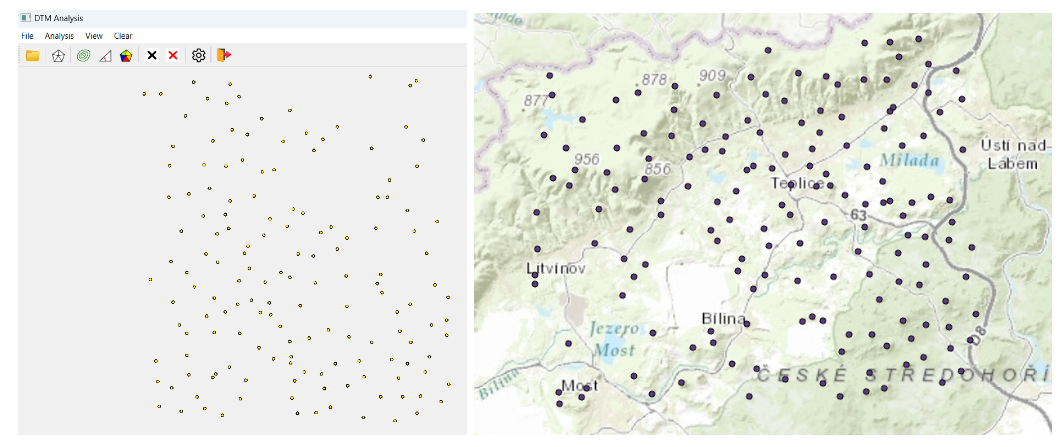
\includegraphics[width=0.9\linewidth]{images/01rozhrani.png}
    \caption{Grafické rozhraní aplikace po načtení bodového mračna (vlevo), stejné body na mapě (vpravo)}
    \label{fig:enter-label}
\end{figure}

Prvním krokem při tvorbě digitálního modelu terénu (DMT) a jeho analýz je vytvoření Delaunay triangulace, jejíž výsledek lze vidět na obrázku 2.

\begin{figure}[h]
    \centering
    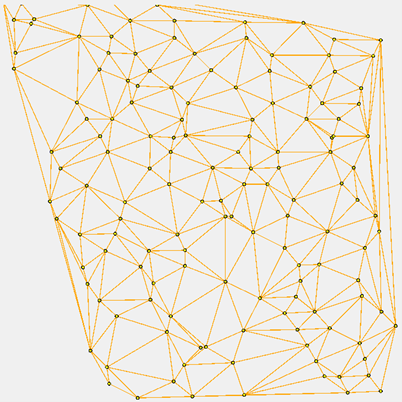
\includegraphics[width=0.4\linewidth]{images/02triangulace.png}
    \caption{Výsledek Delaunay triangulace}
    \label{fig:enter-label}
\end{figure}

\newpage
Z důvodu různé výškové členitosti bodového mračna je potřeba nastavit parametry vykreslování vrstevnic. Defaultní základní interval vrstevnic (ZIV) je 100 m a vrstevnice jsou vykreslovány v rozsahu 0 – 1 610 m. Toto nastavení závisí na výškových poměrech ve zkoumané oblasti. V případě datasetu č.~8 (\textit{test\_8.json}) se jedná o členitou oblast Krušných hor (vlevo), Teplic a Českého Středohoří (vpravo) (obr. 1 vpravo), tudíž správná volba ZIV závisí na účelu (obr. 3). Pokud by se jednalo a oblast s nízkými výškovými rozdíly, ZIV by se muselo správně zvolit. Příliš velký velký interval (např. defaultních 100 m) by v tomto případě nevykreslil žádné vrstevnice. Naopak příliš malý ZIV by zvýraznil malé výškové rozdíly způsobené šumem, v takovém případě je potřeba vrstevnice dostatečně generalizovat. U těchto datasetů s malými výškovými rozdíly není není možné znázornit sklon dostatečně detailně, jelikož je zde malý sklon povrchu (\textit{test\_2.json}, \textit{test\_3.json}) Výsledné vrstevnice při použití dvou zmíněných intervalů lze vidět na obrázku 3.

\begin{figure}[htbp]
    \centering
    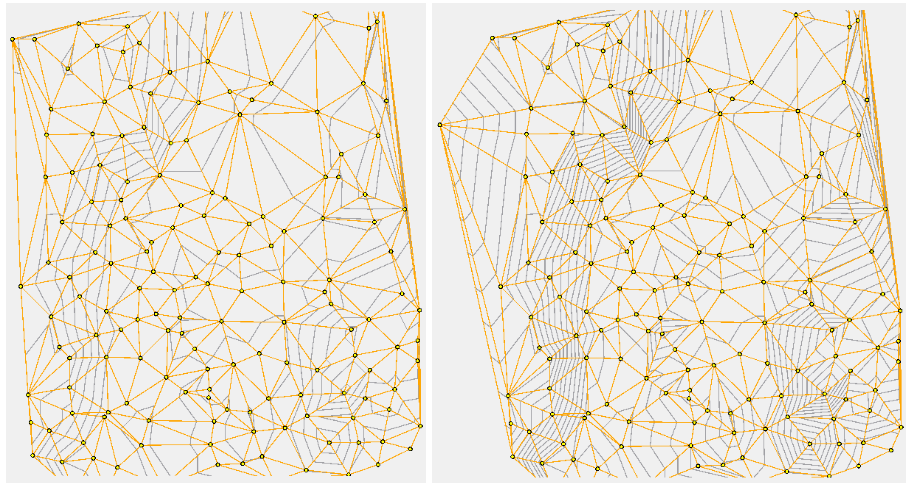
\includegraphics[width=0.8\linewidth]{images/03vrstevnice.png}
    \caption{Různá nastavení základního intervalu vrstevnic, vlevo 100 m, vpravo 50 m}
    \label{fig:enter-label}
\end{figure}

\newpage
Další analyzovanou vlastností námi vytvořeného digitálního modelu terénu byl sklon jednotlivých trojúhelníků, který je znázorněn odstíny šedi. Světlé plochy značí rovinaté oblasti, zatímco tmavé plochy reprezentují strmé oblasti. Výsledek sklonu lze vidět na obrázku 4. 

\begin{figure}[htbp]
    \centering
    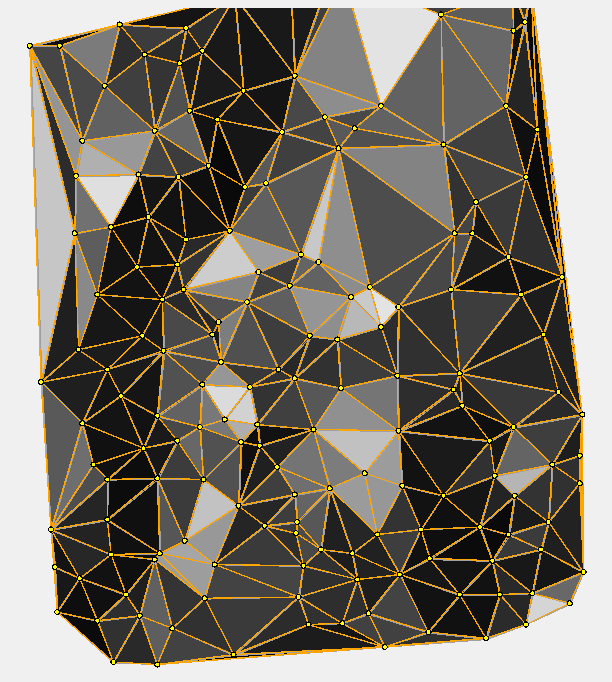
\includegraphics[width=0.4\linewidth]{images/04sklon.png}
    \caption{Výsledek analýzy sklonu}
    \label{fig:enter-label}
\end{figure}

Poslední analyzovanou vlastností digitálního modelu terénu byla orientace vůči světovým stranám, kterou lze vidět na obrázku 5. Pro vizualizaci orientace vůči světovým stranám byla využita barevná stupnice, kterou lze vidět na obrázku 6, kde tyrkysová značí sever, limetková východ, červená jih a fialová západ.

\begin{figure}[htbp]
    \centering
    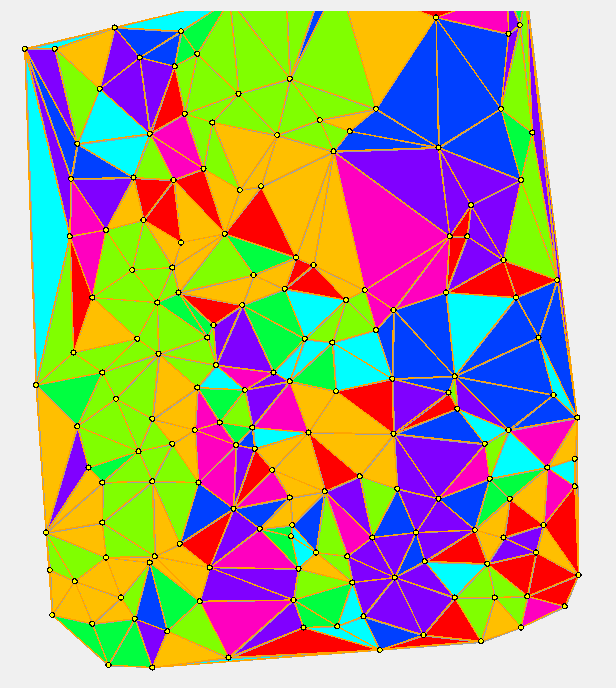
\includegraphics[width=0.4\linewidth]{images/05orientace.png}
    \caption{Výsledek analýzy orientace vůči světovým stranám}
    \label{fig:enter-label}
\end{figure}

\begin{figure}[htbp]
    \centering
    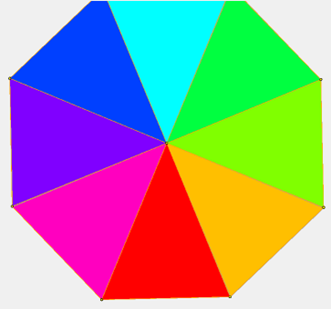
\includegraphics[width=0.3\linewidth]{images/06barvy.png}
    \caption{Barevná stupnice použitá pro vizualizaci orientace}
    \label{fig:enter-label}
\end{figure}

\newpage
Posledním krokem v rámci této úlohy bylo zhodnocení úspěšnosti aplikace. Výsledkem Delaunay triangulace by měly být pokud možno tvarově ideální trojúhelníky. Pokud se podíváme na trojúhelníky vytvořené uprostřed bodového mračna, jako například na obrázku 7, lze vidět, že vytvořené trojúhelníky mají víceméně ideální tvar. Naopak u výsledných krajních trojúhelníků je na první pohled vidět, že mají neideální tvar. Tyto trojúhelníky lze vidět na obrázku 8, kde můžeme pozorovat jejich příliš ostré či naopak příliš tupé úhly.

\begin{figure}[htbp]
    \centering
    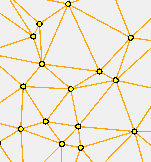
\includegraphics[width=0.2\linewidth]{images/07trojuhelnik.png}
    \caption{Trojúhelníky uprostřed bodového mračna}
    \label{fig:enter-label}
\end{figure}

\begin{figure}[htbp]
    \centering
    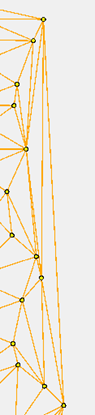
\includegraphics[width=0.1\linewidth]{images/08trojuhelnik_okraj.png}
    \caption{Trojúhelníky na okraji bodového mračna}
    \label{fig:enter-label}
\end{figure}

\newpage
Vrstevnice byly vytvořeny pomocí lineární interpolace a proto úplně stoprocentně neodpovídají skutečnosti. Jak lze vidět na obrázku 9, na některých míst vznikají lomené čáry, které ve skutečnosti mají být spojité křivky jdoucí do oblouků. V námi vytvořené aplikaci také nejspíše nedojde k vykreslení velmi jemných detailů v terénu.

\begin{figure}[htbp]
    \centering
    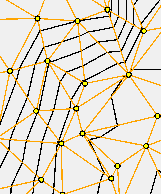
\includegraphics[width=0.3\linewidth]{images/09detail_vrstevnic.png}
    \caption{Detail výsledných vrstevnic}
    \label{fig:enter-label}
\end{figure}

Při detailnější analýze výsledného sklonu lze konstatovat, že výsledek odpovídá skutečnosti. V oblastech většího množství vrstevnic (jako tomu je například na obrázku 10) je barva sklonu tmavší, zatímco v oblastech, kde se nachází velmi málo vrstevnic nebo dokonce žádné (jako na obrázku 11) je sklon znázorněn světlou barvou.

\begin{figure}[htbp]
    \centering
    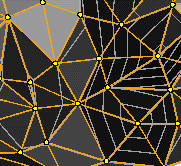
\includegraphics[width=0.3\linewidth]{images/10sklon.png}
    \caption{Výsledný sklon ve strmější oblasti}
    \label{fig:enter-label}
\end{figure}

\begin{figure}[htbp]
    \centering
    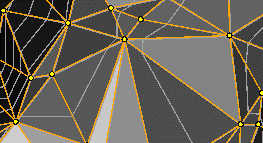
\includegraphics[width=0.3\linewidth]{images/11sklon.png}
    \caption{Výsledný sklon v rovinatější oblasti}
    \label{fig:enter-label}
\end{figure}

\newpage
Výsledná vizualizace orientace terénu vůči světovým stranám je detailní vzhledem k tomu, že došlo k~použití osmi světových stran místo čtyř.  Základní směry (sever, východ, jih, západ) jsou tedy doplněny o severovýchod, jihovýchod, jihozápad a severozápad. Na obrázku 12 lze vidět detailní výsledek analýzy orientace. 

\begin{figure}[htbp]
    \centering
    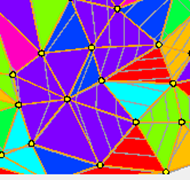
\includegraphics[width=0.3\linewidth]{images/12orientace.png}
    \caption{Detail výsledné orientace vůči světovým stranám}
    \label{fig:enter-label}
\end{figure}

Při použití algoritmu 2D Delaunay triangulace mohou nastat problémy ve znázorňování určitých částí terénu. Obecně se hůře bude znázorňovat velmi členitý terénu s jemnými detaily, jelikož by ke správné reprezentaci terénu bylo potřeba velké množství bodů. Při nedostatečném množství bodů dochází ke vzniku příliš velkých trojúhelníků a tedy k zanedbání malých terénních útvarů. Z důvodu malého množství bodů se například u testovacího souboru č. 8 nejsou znázorněné detailní terénní tvary. Například povrchový důl Bílina není vůbec zobrazen nebo Krušných hor vypadají jako stolová hora. Vrcholy Českého středohoří vypadají jako pyramidy, také z důvodu lineární interpolace vrstevnic (obr. 10). Další problém může nastat při znázorňování hřbetů, údolí, říčních sítí či obecně všech liniových prvků. Pokud jsou body rozmístěny po zájmové oblasti nehomogenně, může interpolace vyústit v nepřesnou reprezentaci strmých svahů. 

\section{Závěr}
V rámci této úlohy došlo k vytvoření aplikace, ve které lze z bodového mračna vytvořit digitální model terénu (DMT). Nad vytvořeným modelem lze vytvořit vrstevnice nebo provádět analýzy jako je sklon a orientace terénu vůči světovým stranám. V této úloze bylo dále popsáno zhodnocení úspěšnosti aplikace, přičemž bylo konstatováno, že aplikace funguje správně. Výpočet vrstevnic byl proveden pomocí lineární interpolace, což by znamenalo, že by se hodnoty nadmořské výšky v celém území měnily lineárně. To se však v přírodě neděje, avšak tento výpočet je nejjednodušší. Detailnější analýzu by bylo možné provést v případě, že by bylo k dispozici mnohem větší množství bodů. Došlo by tak ke znázornění i menších terénním útvarů. 

\section{Zdroje}
CZUK (2024): Stahovací služba WFS - Bodová pole. 

\noindent https://ags.cuzk.cz/arcgis/services/BodovaPole/MapServer/WFSServer? (30. 5. 2024).

\end{spacing}
\end{document}